\subsection{Why does bureaucracy exist? Can't we just do the work?}

Monarchies and dictatorships the rely on a single decider. A simpler model to understand, but difficult to handle all the edge cases for large society. 

Political representatives are an easier to understand concept because it's just one person acting in that behalf of other people.
In contrast emergent behavior of bureaucracy is more difficult to understand. TODO: why not make the entire system out of politicians?

TODO: thought experiment: 
What if everybody in a bureaucracy were the same?
What if everybody in a bureaucracy had a different opinion?


The short answer is that bureaucracy is a response to the complexity of a problem being solved. To see why that is, let's start simple and then increase the complexity. 

The minimal scenario to start from is to imagine a single person working on a single task that does not last long (a few minutes), is relatively easy (cognitively and physically and emotionally), and does not recur. In that situation, building consensus is irrelevant and no process is required. 

Most of what you do occurs outside those limits and thus incurs some concept of \gls{process} (breaking a task into subtasks). Staying with the one-person constraint, a complex task can benefit from being broken into subtasks. Sometimes the order of the subtasks matters, so we need to track the dependencies. A recurring multi-step process with documentation is starting to have features of bureaucracy, but lacks the need for consensus. 

If one person lacks the skills relevant to a multi-step process, they may engage another person to help. The interaction may be informal (anarchy) or formalized in a contract (\href{https://en.wikipedia.org/wiki/Libertarianism}{libertarian}). If the parties working on the task fail to reach consensus, what is the recourse? Options include physical violence, threats, or involving a third party (e.g., a court with lawyers and judges). 


The bureaucrat's identity is subsumed into service for the organization they are part of. At the same time, bureaucracy enables the bureaucrat to amplify their presence by being part of a larger organization. A bureaucrat can accomplish more as part of an organization than by working alone. Sometimes the cost of being part of the organization exceeds the force multiplier of working together. 

% https://graphthinking.blogspot.com/2021/09/why-is-everything-so-hard-in-large.html

What if we completely avoided bureaucracy? That question is better worded by replacing ``bureaucracy" with ``coordination of stakeholders". If you avoid coordination of stakeholders, you either are constrained to only work on tasks that involve one person, or you get is random (uncoordinated) interactions. 

What if we minimized bureaucracy? Again, try replacing ``bureaucracy" in that question with ``coordination of stakeholders". The goal of ``minimizing coordination" probably isn't the real objective. To be more precise, a specific objective might be ``minimize time spent executing the task" (which takes a lot of coordination prior to the task execution) or ``minimize the level of distraction to stakeholders" (chunk the coordination time). Another strategy for minimizing bureaucracy is to reduce the number of stakeholders involved. For a given task complexity, this means having smarter people who have more skills. 

\begin{figure}
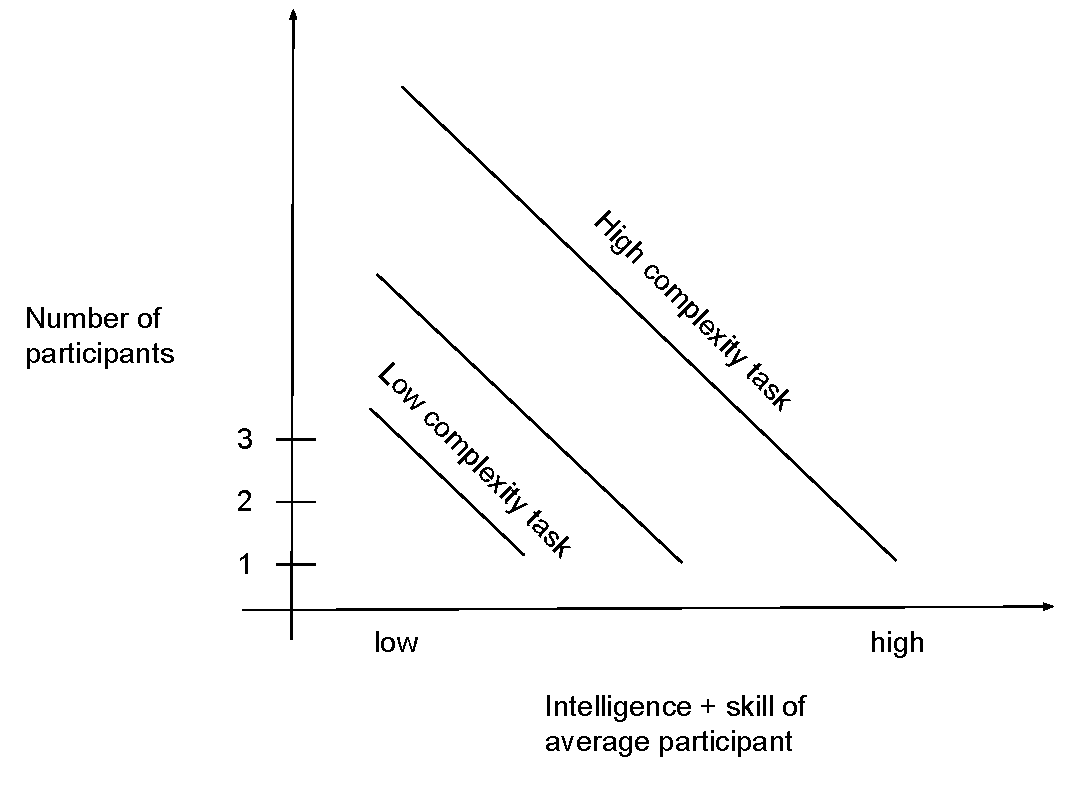
\includegraphics[width=0.8\textwidth]{images/people-per-task-for-skill-level.pdf}
\caption{Three levels of task complexity are shown. As task complexity increases, the size of the team needs to grow. The growth may be less if the team members are brilliant. Those brilliant people cost more and there are fewer of them available.}
\end{figure}
